\appendix
\section{Detailed Software Plan Per Module}
\subsection{Main Unit}
\createfiguresw{0.50\textwidth}{../Detailed-Software-Plan-Per-Module/Figures/main-unit-main-function.png}{Main Unit Main Function Flowchart}{fig:main-unit-main-function-flowchart}
\createfiguresw{0.54\textwidth}{../Detailed-Software-Plan-Per-Module/Figures/main-unit-rtc-isr.png}{Main Unit RTC ISR Flowchart}{fig:main-unit-rtc-isr-flowchart}
\createfigurew{../Detailed-Software-Plan-Per-Module/Figures/main-unit-bluetooth-isr.png}{Main Unit Bluetooth ISR Flowchart}{fig:main-unit-bluetooth-isr-flowchart}
\begin{landscape}
\begin{figure}[!ht]
\begin{center}
  \begin{subfigure}[b]{0.6\textwidth}
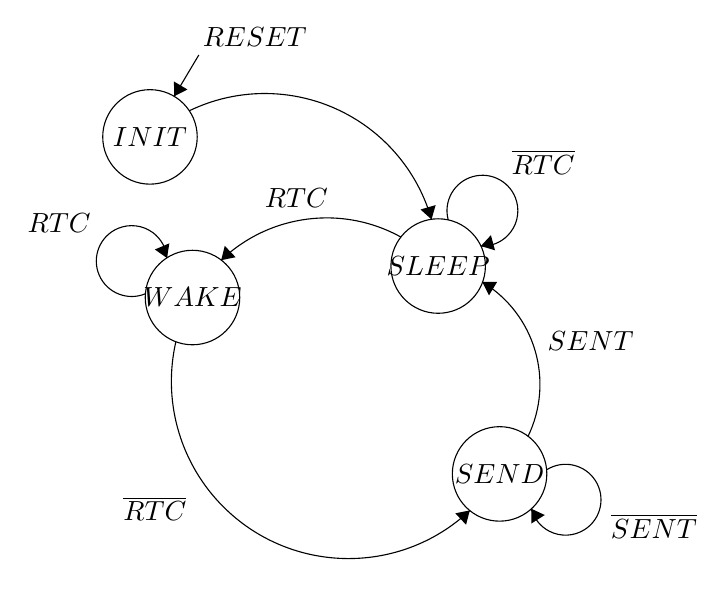
\begin{tikzpicture}[scale=0.2]
\tikzstyle{every node}+=[inner sep=0pt]
\draw [black] (36.8,-8) circle (3);
\draw (36.8,-8) node {$INIT$};
\draw [black] (55.1,-16.2) circle (3);
\draw (55.1,-16.2) node {$SLEEP$};
\draw [black] (39.5,-18.2) circle (3);
\draw (39.5,-18.2) node {$WAKE$};
\draw [black] (59,-29.4) circle (3);
\draw (59,-29.4) node {$SEND$};
\draw [black] (39.9,-2.8) -- (38.34,-5.42);
\draw (43.45,-2.3) node [above] {$RESET$};
\fill [black] (38.34,-5.42) -- (39.18,-4.99) -- (38.32,-4.48);
\draw [black] (39.29,-6.344) arc (115.82686:15.90003:11.012);
\fill [black] (54.68,-13.24) -- (54.94,-12.33) -- (53.98,-12.61);
\draw [black] (55.741,-13.281) arc (195.34019:-92.65981:2.25);
\draw (61.76,-10.43) node [above] {$\overline{RTC}$};
\fill [black] (57.81,-14.93) -- (58.71,-15.2) -- (58.45,-14.24);
\draw [black] (41.319,-15.829) arc (133.66152:60.95:9.714);
\fill [black] (41.32,-15.83) -- (42.24,-15.64) -- (41.55,-14.92);
\draw (46.1,-12.5) node [above] {$RTC$};
\draw [black] (57.903,-17.214) arc (58.79222:-25.87219:7.596);
\fill [black] (57.9,-17.21) -- (58.33,-18.06) -- (58.85,-17.2);
\draw (62.02,-20.97) node [right] {$SENT$};
\draw [black] (57.113,-31.721) arc (-46.74993:-192.99266:11.248);
\fill [black] (57.11,-31.72) -- (56.19,-31.9) -- (56.87,-32.63);
\draw (37.11,-30.8) node [below] {$\overline{RTC}$};
\draw [black] (61.977,-29.145) arc (122.62938:-165.37062:2.25);
\draw (66.04,-32.72) node [right] {$\overline{SENT}$};
\fill [black] (61.01,-31.61) -- (61.02,-32.55) -- (61.87,-32.01);
\draw [black] (36.522,-17.955) arc (293.03624:5.03624:2.25);
\draw (33.07,-13.46) node [left] {$RTC$};
\fill [black] (37.88,-15.69) -- (38.03,-14.76) -- (37.11,-15.15);
\end{tikzpicture}
\caption{Main Unit Functional State Diagram}
\label{fig:main-unit-fsd-img}
  \end{subfigure}
  \begin{subfigure}[b]{0.5\textwidth}
      \begin{tabular}{c|ccc}
        STATE&\multicolumn{3}{c}{OUTPUTS}\\
        \hline
        &&&\\
        INIT&$RESET$&$\overline{RTC}$&$\overline{SENT}$\\
        SLEEP&$\overline{RESET}$&$\overline{RTC}$&$\overline{SENT}$\\
        WAKE&$\overline{RESET}$&$RTC$&$\overline{SENT}$\\
        SEND&$\overline{RESET}$&$\overline{RTC}$&$\overline{SENT}$\\
      \end{tabular}
      \caption{Main Unit Functional State Diagram: State and Outputs}
      \label{fig:main-unit-fsd-state-outputs}
  \end{subfigure}
  \begin{subfigure}[b]{0.5\textwidth}
   \begin{tabular}{|c|}
    \hline
     Output List\\
    \hline
     RESET = Power on Reset\\
     SLEEP = MCU is in LPM4\\
     WAKE = RTC Timer turned on MCU\\
     SEND = Bluetooth module is sending data\\
    \hline
   \end{tabular}
      \caption{Main Unit Functional State Diagram: Output List}
      \label{fig:main-unit-fsd-outputs-list}
  \end{subfigure}
\end{center}
\caption{Main Unit Functional State Diagram}
\label{fig:main-unit-fsd}
\end{figure}
\end{landscape}

\newpage
\createfigurew{../Detailed-Software-Plan-Per-Module/Figures/main-unit-main-function-pseudo-code.png}{Main Unit Main Function Pseudo Code}{fig:main-unit-main-function-pseudo-code}
\createfigurew{../Detailed-Software-Plan-Per-Module/Figures/main-unit-rtc-isr-pseudo-code.png}{Main Unit RTC ISR Pseudo Code}{fig:main-unit-rtc-isr-pseudo-code}
\createfigurew{../Detailed-Software-Plan-Per-Module/Figures/main-unit-bluetooth-isr-pseudo-code.png}{Main Unit Bluetooth ISR Pseudo Code}{fig:main-unit-bluetooth-isr-pseudo-code}
\subsection{Sub Unit}
\createfiguresw{0.50\textwidth}{../Detailed-Software-Plan-Per-Module/Figures/sub-unit-main-function.png}{Sub Unit Main Function Flowchart}{fig:sub-unit-main-function-flowchart}
\createfiguresw{0.75\textwidth}{../Detailed-Software-Plan-Per-Module/Figures/sub-unit-rtc-isr.png}{Sub Unit RTC ISR Flowchart}{fig:sub-unit-rtc-isr-flowchart}
\createfiguresw{0.75\textwidth}{../Detailed-Software-Plan-Per-Module/Figures/sub-unit-bluetooth-isr.png}{Sub Unit Bluetooth ISR Flowchart}{fig:sub-unit-bluetooth-isr-flowchart}
\begin{landscape}
\begin{figure}[!ht]
\begin{center}
  \begin{subfigure}{\textwidth}
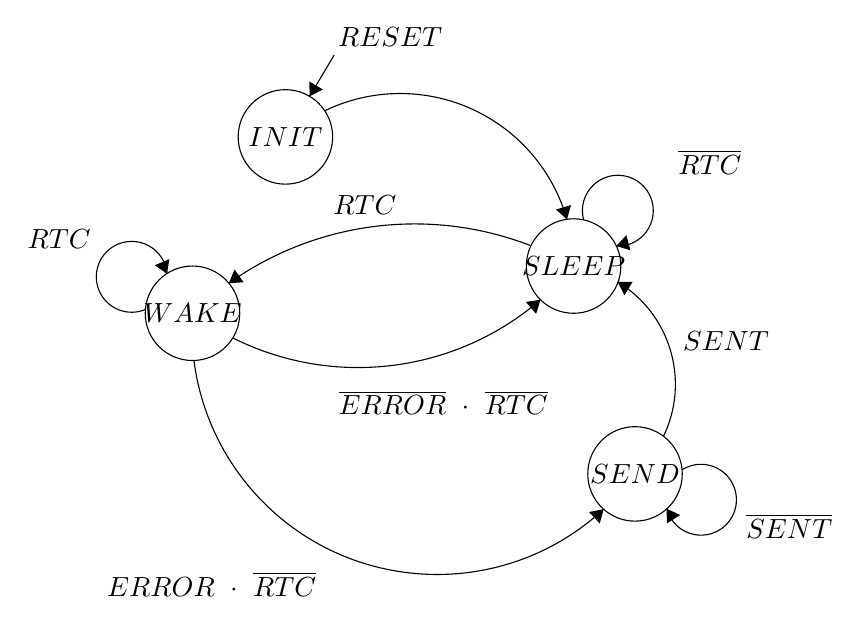
\begin{tikzpicture}[scale=0.2]
\tikzstyle{every node}+=[inner sep=0pt]
\draw [black] (36.8,-8) circle (3);
\draw (36.8,-8) node {$INIT$};
\draw [black] (55.1,-16.2) circle (3);
\draw (55.1,-16.2) node {$SLEEP$};
\draw [black] (30.9,-19.2) circle (3);
\draw (30.9,-19.2) node {$WAKE$};
\draw [black] (59,-29.4) circle (3);
\draw (59,-29.4) node {$SEND$};
\draw [black] (39.9,-2.8) -- (38.34,-5.42);
\draw (43.45,-2.3) node [above] {$RESET$};
\fill [black] (38.34,-5.42) -- (39.18,-4.99) -- (38.32,-4.48);
\draw [black] (39.29,-6.344) arc (115.82686:15.90003:11.012);
\fill [black] (54.68,-13.24) -- (54.94,-12.33) -- (53.98,-12.61);
\draw [black] (55.741,-13.281) arc (195.34019:-92.65981:2.25);
\draw (63.76,-10.43) node [above] {$\overline{RTC}$};
\fill [black] (57.81,-14.93) -- (58.71,-15.2) -- (58.45,-14.24);
\draw [black] (33.209,-17.289) arc (125.38493:68.74853:20.376);
\fill [black] (33.21,-17.29) -- (34.15,-17.23) -- (33.57,-16.42);
\draw (41.85,-12.97) node [above] {$RTC$};
\draw [black] (57.903,-17.214) arc (58.79222:-25.87219:7.596);
\fill [black] (57.9,-17.21) -- (58.33,-18.06) -- (58.85,-17.2);
\draw (62.02,-20.97) node [right] {$SENT$};
\draw [black] (53.003,-18.341) arc (-49.24761:-116.61893:17.757);
\fill [black] (53,-18.34) -- (52.07,-18.48) -- (52.72,-19.24);
\draw (46.82,-24.07) node [below] {$\overline{ERROR}\mbox{ }\cdot\mbox{ }\overline{RTC}$};
\draw [black] (57.009,-31.638) arc (-47.17822:-172.72249:15.564);
\fill [black] (57.01,-31.64) -- (56.08,-31.82) -- (56.76,-32.55);
\draw (32.12,-35.61) node [below] {$ERROR\mbox{ }\cdot\mbox{ }\overline{RTC}$};
\draw [black] (61.977,-29.145) arc (122.62938:-165.37062:2.25);
\draw (66.04,-32.72) node [right] {$\overline{SENT}$};
\fill [black] (61.01,-31.61) -- (61.02,-32.55) -- (61.87,-32.01);
\draw [black] (27.922,-18.955) arc (293.03624:5.03624:2.25);
\draw (24.47,-14.46) node [left] {$RTC$};
\fill [black] (29.28,-16.69) -- (29.43,-15.76) -- (28.51,-16.15);
\end{tikzpicture}
\caption{Sub Unit Functional State Diagram}
\label{fig:sub-unit-fsd-diagram}
  \end{subfigure}
  \begin{subfigure}[b]{0.5\textwidth}
      \begin{tabular}{c|cccc}
        STATE&\multicolumn{3}{c}{OUTPUTS}\\
        \hline
        &&&\\
        INIT&$RESET$&$\overline{RTC}$&$\overline{SENT}$&$\overline{ERROR}$\\
        SLEEP&$\overline{RESET}$&$\overline{RTC}$&$\overline{SENT}$&$\overline{ERROR}$\\
        WAKE&$\overline{RESET}$&$RTC$&$\overline{SENT}$&$\overline{ERROR}$\\
        SEND&$\overline{RESET}$&$\overline{RTC}$&$\overline{SENT}$&$ERROR$\\
      \end{tabular}
      \caption{Sub Unit Functional State Diagram: State and Outputs}
      \label{fig:sub-unit-fsd-state-outputs}
  \end{subfigure}
  \begin{subfigure}[b]{0.5\textwidth}
   \begin{tabular}{|c|}
    \hline
     Output List\\
    \hline
     RESET = Power on Reset\\
     SLEEP = MCU is in LPM4\\
     WAKE = RTC Timer turned on MCU\\
     SEND = Bluetooth module is sending data\\
     ERROR = Temperature or Age Related Error Detected\\
    \hline
   \end{tabular}
      \caption{Sub Unit Functional State Diagram: Output List}
      \label{fig:sub-unit-fsd-outputs-list}
  \end{subfigure}
\caption{Sub Unit Functional State Diagram}
\label{fig:sub-unit-fsd}
\end{center}
\end{figure}

\createfigurew{../Detailed-Software-Plan-Per-Module/Figures/sub-unit-main-function-pseudo-code.png}{Sub Unit Main Function Pseudo Code}{fig:sub-unit-main-function-pseudo-code}
\createfigurew{../Detailed-Software-Plan-Per-Module/Figures/sub-unit-rtc-isr-pseudo-code.png}{Sub Unit RTC ISR Pseudo Code}{fig:sub-unit-rtc-isr-pseudo-code}
\createfigurew{../Detailed-Software-Plan-Per-Module/Figures/sub-unit-bluetooth-isr-pseudo-code.png}{Sub Unit Bluetooth ISR Pseudo Code}{fig:sub-unit-bluetooth-isr-pseudo-code}
\begin{minted}[breaklines,breakanywhere]{C}
#include <msp430.h> 
#include <temperatureSensor.h>
#include <bluetooth.h>

typedef enum
{
    OLD, FROZEN, COLD, WARM, HOT, TRASH, NONE
} ERROR;

char*ERROR_STRING[7] = {
    "OLD",
    "FROZEN",
    "COLD",
    "WARM",
    "HOT",
    "TRASH",
    "NONE"
};

char LOT[30] = "ABCDEFGHIJKLMNOPQRSTUVWXYZ1234";

void checkExpDate();
void raiseError(ERROR err);


unsigned int currHour = 0;
const unsigned int expDateHours = 17520;
ERROR error = NONE;

int main(void)
{
    WDTCTL = WDTPW | WDTHOLD;	// stop watchdog timer

    P6SEL |= BIT7;
    ADC12CTL0 |= ADC12SHT0_15 + ADC12ON;
    ADC12CTL1 = ADC12SHP;
    ADC12MCTL0 |= ADC12INCH_7 + ADC12SREF_7;
    ADC12IE |= BIT0;
    ADC12CTL0 |= ADC12ENC;


//    RTCCTL01 = RTCTEVIE + RTCSSEL_2 + RTCTEV_0; // Counter Mode, RTC1PS, 8-bit ovf
//                                              // overflow interrupt enable
//    RTCPS0CTL = RT0PSDIV_2;                   // ACLK, /8, start timer
//    RTCPS1CTL = RT1SSEL_2 + RT1PSDIV_3;       // out from RT0PS, /16, start timer
    RTCCTL0 |= RTCTEVIE + RTCRDYIE;
    RTCCTL1 |= RTCTEV_0 + RTCBCD;

    P2DIR |= BIT0;
    P2OUT &= ~BIT0;

    P3SEL = BIT4 + BIT5;
    UCA0CTL1 |= UCSWRST;
    UCA0CTL1 |= UCSSEL_2;
    UCA0BR0 = 109;
    UCA0BR1 = 0x00;
    UCA0MCTL = UCBRS_2+UCBRF_0;
    UCA0CTL1 &= ~UCSWRST;
    UCA0IE |= UCTXIE + UCRXIE;
    __enable_interrupt();

    executeAT_Command("AT",NULL,NULL);
    __bis_SR_register(LPM3_bits);
}

#pragma vector=RTC_VECTOR
__interrupt void RTC_ISR(void)
{

}

#if defined(__TI_COMPILER_VERSION__) || defined(__IAR_SYSTEMS_ICC__)
#pragma vector=RTC_VECTOR
__interrupt void RTC_ISR(void)
#elif defined(__GNUC__)
void __attribute__ ((interrupt(RTC_VECTOR))) RTC_ISR (void)
#else
#error Compiler not supported!
#endif
{
  switch(__even_in_range(RTCIV,16))
  {
    case 0: break;                          // No interrupts
    case 2: break;                          // RTCRDYIFG
    case 4:                                 // RTCEVIFG
        currHour += 1;
        unsigned int i = 0;
        for (; i < TEMPBUFSIZE; i++)
        {
            ADC12CTL0 |= ADC12SC;
            while (ADC12CTL1 & ADC12BUSY);
            voltage = ADC12MEM0;
            tempts[tempindex] = (voltage) / 10.0;
            tempindex = (++tempindex) % TEMPBUFSIZE;
        }
        float average = average_celsius();
        if (average < 2 || average > 8)
        {
            if (average <= 0)
            {
                raiseError(FROZEN);
            }
            else if (average > 0 && average < 2)
            {
                raiseError(COLD);
            }
            else if (average > 8 && average < 15)
            {
                raiseError(WARM);
            }
            else if (average >= 15 && average < 30)
            {
                raiseError(WARM);
            }
            else
            {
                raiseError(TRASH);
            }
        }
        checkExpDate();
        if (error == NONE)
        {
            P2OUT &= ~BIT0;
        }

        __bic_SR_register_on_exit(LPM3_bits);   // Exit active CPU
      break;
    case 6: break;                          // RTCAIFG
    case 8: break;                          // RT0PSIFG
    case 10: break;                         // RT1PSIFG
    case 12: break;                         // Reserved
    case 14: break;                         // Reserved
    case 16: break;                         // Reserved
    default: break;
  }
}

void checkExpDate()
{
    if (currHour > expDateHours)
    {
        error = OLD;
    }
}

void raiseError(ERROR err)
{
    error = err;
    P2OUT |= BIT0;
    sprintf(BTTXBUF,"%s %s",LOT,ERROR_STRING[err]);
    UCA0IE |= UCTXIE;

}

#pragma vector=USCI_A0_VECTOR
__interrupt void USCI_A0_ISR(){
    switch(__even_in_range(UCA0IV,4)){
    case 0: break;
    case 2:
        if (rxcharindex < BTBUFSIZE && rxcharindex < strlen(BTRXBUF)){
            UCA0RXBUF = BTRXBUF[rxcharindex];
            rxcharindex += 1;
        }
        else {
            resetBuffer(BTRXBUF);
            rxcharindex = 0;
        }
        break;
    case 4:
        if (txcharindex < BTBUFSIZE && txcharindex < strlen(BTTXBUF)){
            UCA0TXBUF = BTTXBUF[txcharindex];
            txcharindex += 1;
        }
        else {
            txcharindex = 0;
            UCA0IE &= ~UCTXIE;
        }
        break;
    default: break;
    }
}
\end{minted}
